Pick a portfolio at random.  That sounds easy: draw some numbers, turn them
into weights, and make them sum to one.  But what should ``at random'' mean?
The answer matters because an innocent-looking shortcut can quietly favor
some portfolios over others.

Suppose a portfolio has $D$ assets.  Its long-only, fully invested weights
lie on the probability simplex
\[
\Delta_{D-1}=\left\{\boldsymbol{p}\in\mathbb{R}^D:
p_i\geq 0,\ \sum_{i=1}^D p_i=1\right\}.
\]
Here is the tempting shortcut: draw $D$ independent
Uniform$(0,1)$ values and divide them by their sum.  This lands on
$\Delta_{D-1}$, but it is not uniform there: it puts too much mass near the
centroid and too little near the vertices~\cite{devroye1986,smithtromble2004}.
The bias is specific to normalized uniform draws.  For quasi-Monte Carlo
(QMC) sampling, this construction also spends $D$ cube coordinates on a
$(D-1)$-dimensional target.

\paragraph{How do we remove the hidden bias?}
QMCPy's~\cite{QMCPy} \code{SimplexUniform} supplies the needed
cube-to-simplex map developed by \cite{pillardscools2005}.  It returns a point
in the $(D-1)$-dimensional corner simplex
\[
K_{D-1}=\left\{\boldsymbol{w}\in\mathbb{R}^{D-1}:
w_i\geq 0,\ \sum_{i=1}^{D-1} w_i\leq 1\right\}.
\]
The two representations correspond through the bijection
\[
\boldsymbol{w}\longmapsto
\boldsymbol{p}=\left(w_1,\ldots,w_{D-1},1-\sum_{i=1}^{D-1} w_i\right)
\in\Delta_{D-1}.
\]
Thus, appending the final coordinate gives a point uniformly distributed on
$\Delta_{D-1}$, equivalently a Dirichlet$(1,\ldots,1)$ vector.  A sampler
for $D$ portfolio weights needs only $D-1$ cube coordinates.

The public \code{transform\_points} method makes the transformation explicit
and lets several methods use the same pre-generated cube points:

\lstinputlisting[style=Python, firstline=9, lastline=15]{PortfolioSimplex/code/simplex_bias.py}

\begin{figure}[H]
\centering
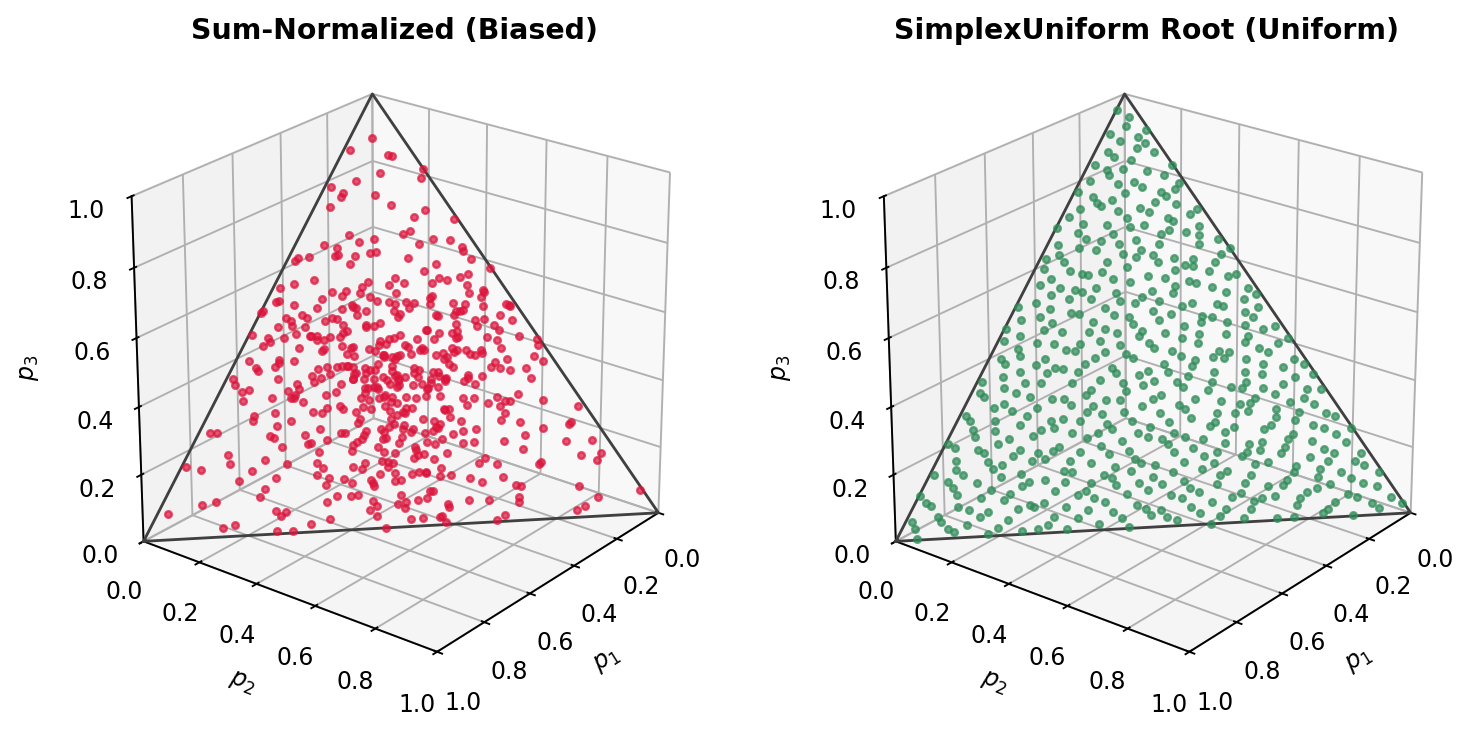
\includegraphics[width=0.95\linewidth]{PortfolioSimplex/images/simplex_bias.png}
\caption{512 Sobol points mapped onto the probability 2-simplex. Left:
normalizing three uniform coordinates concentrates points toward the center.
Right: the \code{root} simplex transform consumes two cube coordinates and
produces uniform simplex weights, including the implicit third weight.}
\end{figure}

\paragraph{Five maps to a uniform simplex.}
Internally, \code{SimplexUniform} first maps $[0,1]^{D-1}$ to the ordered simplex
$T_{D-1}=\{0\leq x_1\leq\cdots\leq x_{D-1}\leq1\}$, then converts the ordered
coordinates to the full probability-simplex weights,
\[
p_1=x_1,\qquad p_i=x_i-x_{i-1}\ (2\leq i\leq D-1),\qquad
p_D=1-x_{D-1}.
\]
Why offer five maps if they have the same target distribution?  A QMC rule cares about how the map carries the structure of well-spaced cube points onto the simplex, not only about the distribution of a single point.  The available \code{root},
\code{sort}, \code{shift}, \code{origami}, and \code{mirror} maps are distinct
measure-preserving constructions studied by Pillards and
Cools~\cite{pillardscools2005} and in Pillards' thesis~\cite{pillards2006}.
The 2005 paper gives Shift in two dimensions; Section~4.3 of the 2006 thesis
constructs its higher-dimensional version through an intermediate corner
simplex.  QMCPy's \code{shift} uses the later construction in every dimension,
including two, so it is not pointwise identical to the original 2D map.
\code{mirror} is
implemented only for input dimensions of at most 3.
The \code{sort}, \code{origami}, and \code{mirror} maps are not injective, so
different cube points may have the same image.  QMCPy retains every occurrence
as a multiset (a collection that keeps duplicates): each still carries its
original $1/N$ quadrature weight.
Deleting duplicates would change the QMC rule.

\paragraph{Does every low-discrepancy (LD) sequence behave alike?}
The
\href{https://github.com/QMCSoftware/QMCSoftware/blob/develop/demos/simplex_uniform.ipynb}{SimplexUniform demo}
validates support and moments and demonstrates all five transformations.  Its
interactive figures separate the LD family from the family's
randomization or construction type.  They currently cover Sobol, lattice,
Halton, Faure, Hammersley, Kronecker, and Korobov lattice points---31
family/type combinations in total---and compare their simplex convergence on
a common vertical scale.  Try changing both menus: the geometry of the map
can interact visibly with the structure of the point set.  The interactive
convergence plot uses the linear integrand $\sum_i w_i$; under \code{root},
it depends on only one cube coordinate, which makes this illustration
especially favorable to \code{root}.

\paragraph{What happens when simplex points become portfolios?}
The
\href{https://github.com/QMCSoftware/QMCSoftware/blob/develop/demos/portfolio/portfolio_allocation_demo.ipynb}{Portfolio Allocation demo}
uses the \code{root} transform for every candidate portfolio.  It compares
independent and identically distributed (IID) points
with six LD families---lattice, Sobol, Halton, Faure, Kronecker,
and Korobov lattice---while keeping the target distribution on
$\Delta_{D-1}$ fixed.  Hammersley is deterministic and does not provide the
independent randomizations used for the reported standard errors;
message-passing Monte Carlo (MPMC) needs its optional machine-learning stack
and is too expensive for this particular sweep.  Every sampler is constructed
directly in $D-1$ dimensions.

Candidate weights are scored with a conventional constant-weight objective:
asset log returns derived from the saved price data are converted to simple
returns before computing the portfolio mean and covariance.  A date-matched annual log risk-free rate,
when used, is converted to a daily simple return before subtraction.  This
selection Sharpe ratio answers a different question from the realized
strategy: the in-sample backtest rebalances quarterly, while the out-of-sample
backtest buys and holds, so their weights drift between trades.

The answer is more interesting than a simple leaderboard.  With 32,768
candidate portfolios, the best medium-risk score changes with the asset
universe and the risk-free-rate choice.  For 40 tickers, the seven mean
Sharpe ratios range from 1.269 to 1.277 without the risk-free rate and from
1.170 to 1.179 with it; their standard errors are 0.002--0.004.  Thus IID is
competitive and sometimes best, but the differences are small relative to
the reported replication uncertainty.  The useful lesson lies in the comparison itself: use the same simplex
law and candidate count, and report variation across randomizations.  The
out-of-sample dollar results are also mixed.  That table reports replication
means without standard errors, so it is descriptive and does not establish a
sampler-specific investment edge.

\paragraph{Where can a backtest accidentally lose a dollar?}
Sampling is only half the story.  The backtest must also conserve capital
through data and trading events.  Its fitting and valuation dates are reported separately and use a common
history where required.  As safeguards, under buy-and-hold a late-listed asset's allocation
stays in cash until listing; a temporarily unavailable holding is frozen at
its last traded value; rebalancing redistributes only the tradeable pool; and
stop-loss proceeds move to the remaining eligible assets, or to cash when no
eligible target mass remains.  The reported data have complete price histories
and use no stop loss, so none of these safeguards fires in the demo.  The rules
prevent missing prices or a rebalance boundary from creating or destroying wealth.

The experiment leaves us with a useful question instead of a slogan: when
does the structure of an LD sequence survive a simplex transform strongly
enough to improve the search?  The demos make that
question easier to explore.  They illustrate simplex sampling,
not a production portfolio strategy or investment advice.  The authors are
not financial professionals.
